\documentclass[a4paper, 11pt]{article}

% Nécessaire
\usepackage[french]{babel}
\usepackage[utf8]{inputenc}
\usepackage[T1]{fontenc}
\usepackage{lmodern}
\usepackage{amsmath, amsthm}
\usepackage{amsfonts,amssymb}

% Marge
\usepackage{geometry}
\geometry{margin={2.1cm ,2.1cm}}

% Figures, graphiques
\usepackage{graphicx}
\usepackage{epsfig}
\usepackage{caption}

% Surlignage
\usepackage{alltt}

\usepackage{xcolor}
\usepackage{soul}
\usepackage{color}
\usepackage{colortbl}

% Indicatrice
\usepackage{dsfont}

\usepackage{multirow}
\usepackage{eurosym}
\usepackage{extarrows}


% Titre
\title{Décomposition et saisonnalité}
\author{}
\date{}
 
\begin{document}
 
\maketitle

Ce document a pour objectif de présenter la provenance des femelles qui pondent des œufs. Ce document présente aussi ce que donne l'introduction d'un paramètre de saisonnalité (vers le 15 septembre) dans le modèle.

\section{Décomposition}

On peut voir sur le graphe ci-dessous de quelles femelles proviennent les larves estimées.

\begin{figure}[!h]
\centering
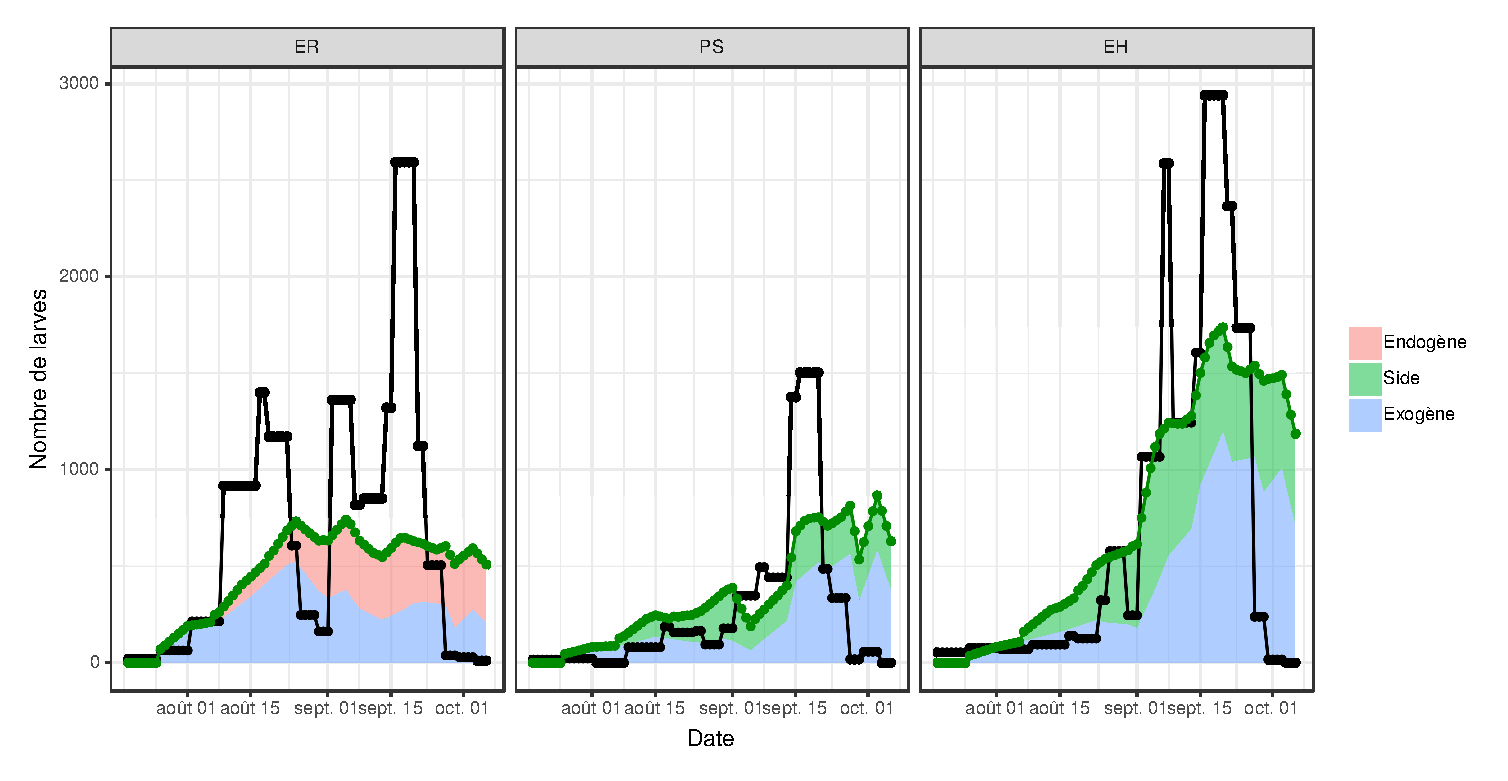
\epsfig{file = plots/ref_decomposed.eps, scale = 0.65}
\caption{Décomposition de la provenance des larves, soit endogène au sous-bloc, soit venant d'un autre sous-bloc, soit exogène au bloc. }
\end{figure}

Les paramètres trouvés sont les suivants
\begin{center}
\begin{tabular}{lllll}
$\gamma$ & $p_m$ & $\mu_{ER}$ & $\mu_{EH}$ & $k$\\
0.04 & 0.6 & 0.58 & 0 & 32
\end{tabular}
\end{center}


\newpage
Si l'on fixe les exogènes à 20 :

\begin{figure}[!h]
\centering
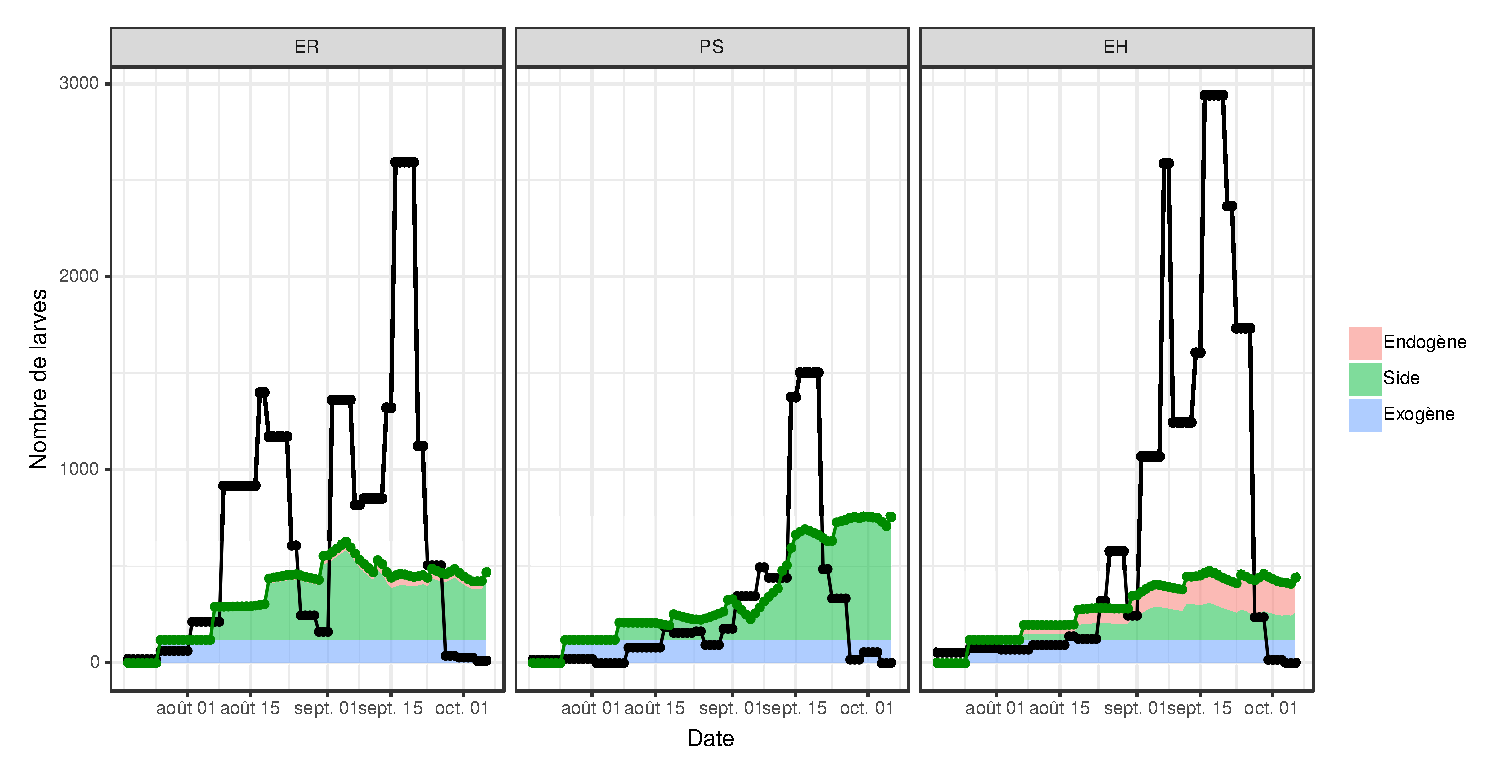
\epsfig{file = plots/noexo_decomposed.eps, scale = 0.65}
\caption{Décomposition de la provenance des larves, soit endogène au sous-bloc, soit venant d'un autre sous-bloc, soit exogène au bloc. }
\end{figure}

Les paramètres trouvés sont les suivants
\begin{center}
\begin{tabular}{llll}
$p_m$ & $\mu_{ER}$ & $\mu_{EH}$ & $k$\\
0.82 & 0.23 & 0.99 & 34
\end{tabular}
\end{center}

\section{Saisonnalité}

Dans cette section, on introduit un paramètre de saisonnalité intervenant sur les femelles à partir du 15 septembre.

\begin{figure}[!h]
\centering
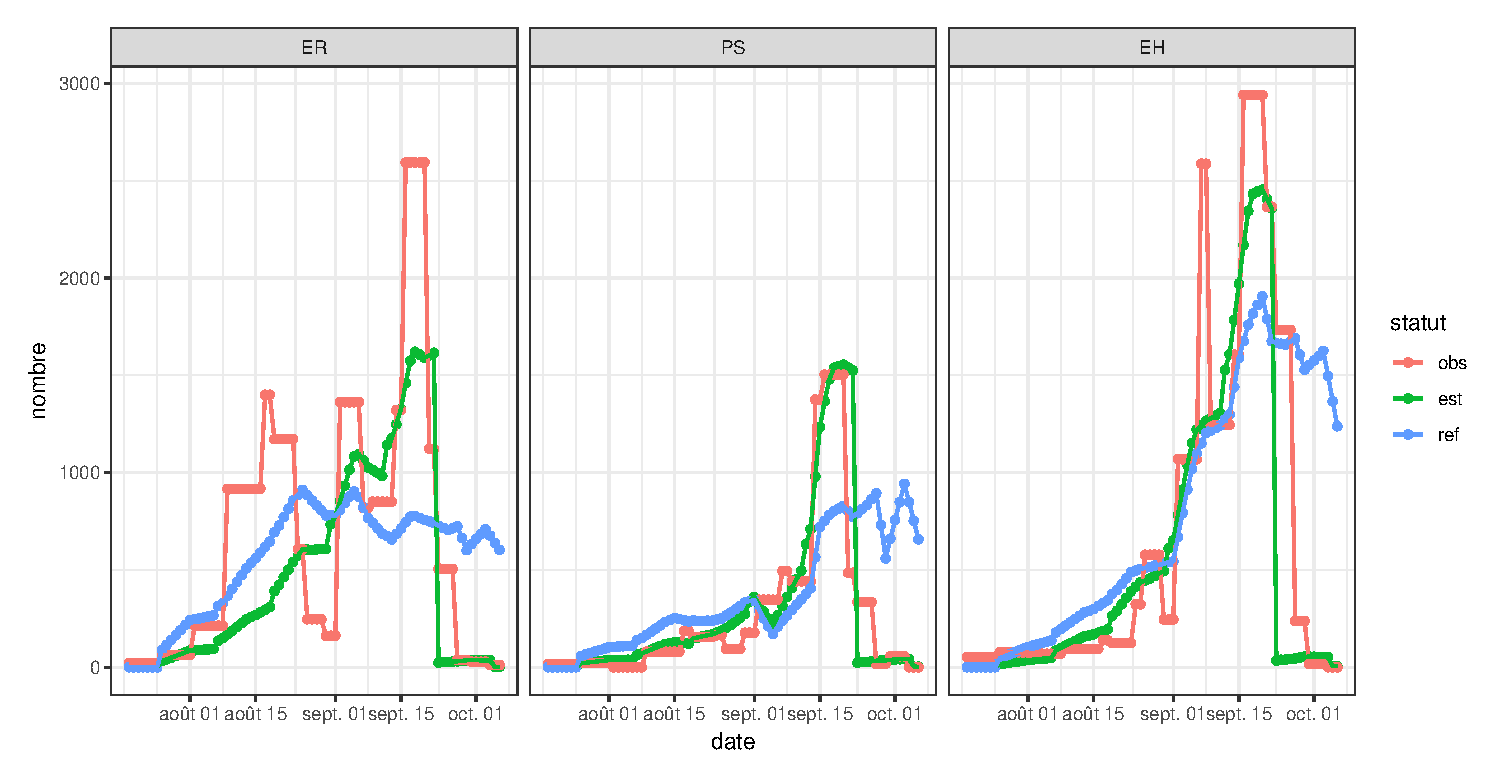
\epsfig{file = plots/saison.eps, scale = 0.65}
\caption{Avec paramètre de saisonnalité}
\end{figure}


On notera $\xi^{end}$ le coefficent par lequel seront multiplié les femelles à partir du 15 septembre. Les paramètres trouvés sont 
\begin{center}
\begin{tabular}{llllll}
$\gamma$ & $p_m$ & $\mu_{ER}$ & $\mu_{EH}$ & $k$ & $\xi^{end}$\\
0.016 & 0.6 & 0.95 & 0.77 & 6.75 & 0.02
\end{tabular}
\end{center}


Si on considère que les exogènes arrivent de façon constante (fixé à 20 femelles). On obtient

\begin{figure}[!h]
\centering
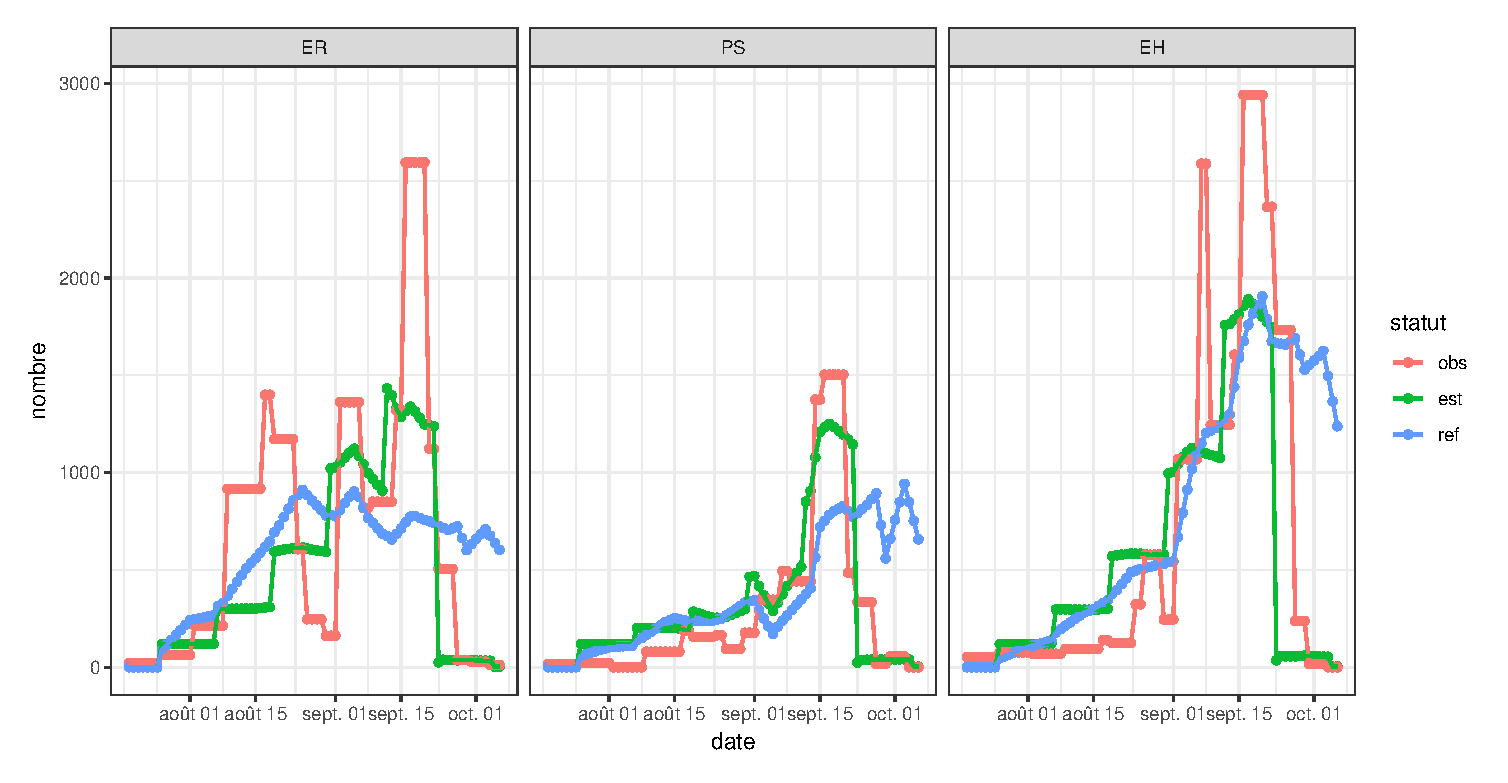
\epsfig{file = plots/saison_noexo.eps, scale = 0.65}
\caption{Avec paramètre de saisonnalité}
\end{figure}

Les paramètres obtenus sont 
\begin{center}
\begin{tabular}{lllll}
 $p_m$ & $\mu_{ER}$ & $\mu_{EH}$ & $k$ & $\xi^{end}$\\
 0.53 & 0.58 & 0.99 & 7.15 & 0.02
\end{tabular}
\end{center}



\end{document}
